\chapter{Grundlagen}
\label{chap:Grundlagen}
Im folgenden Kapitel werden die Grundlagen der Arbeit, insbesondere im Hinblick auf die gewählten Ansätze, beschrieben. Begonnen wird mit den angewendeten Methoden, gefolgt von einer Beschreibung bestehender Systeme, den Daten und den durchgeführten Vorverarbeitungen.

	\section{Autoencoder}
	\label{sec:ConvolutionalAutoencoder}		
	Autoencoder \cite{D.E.Rumelhart.1987} sind Werkzeuge, die insbesondere zum Finden von Repräsentationen eingesetzt werden. Dabei komprimieren sie die Eingabe in einen niedrigdimensionaleren Raum und rekonstruieren aus diesem die Eingabe. Konkret besteht ein Autoencoder aus drei Teilen: dem Encoder, dem Codelayer und dem Decoder. In der einfachsten Form besteht ein Autoencoder aus einer Eingabeschicht, einer versteckten Schicht und eine Ausgabeschicht, siehe Abbildung \ref{img:SchemaCAE}. Sie können nach \cite{Hinton.2006} mit mehreren Schichten, also mit \textit{tiefen Architekturens} genutzt werden. 
	\begin{figure}[h]
		\centering
		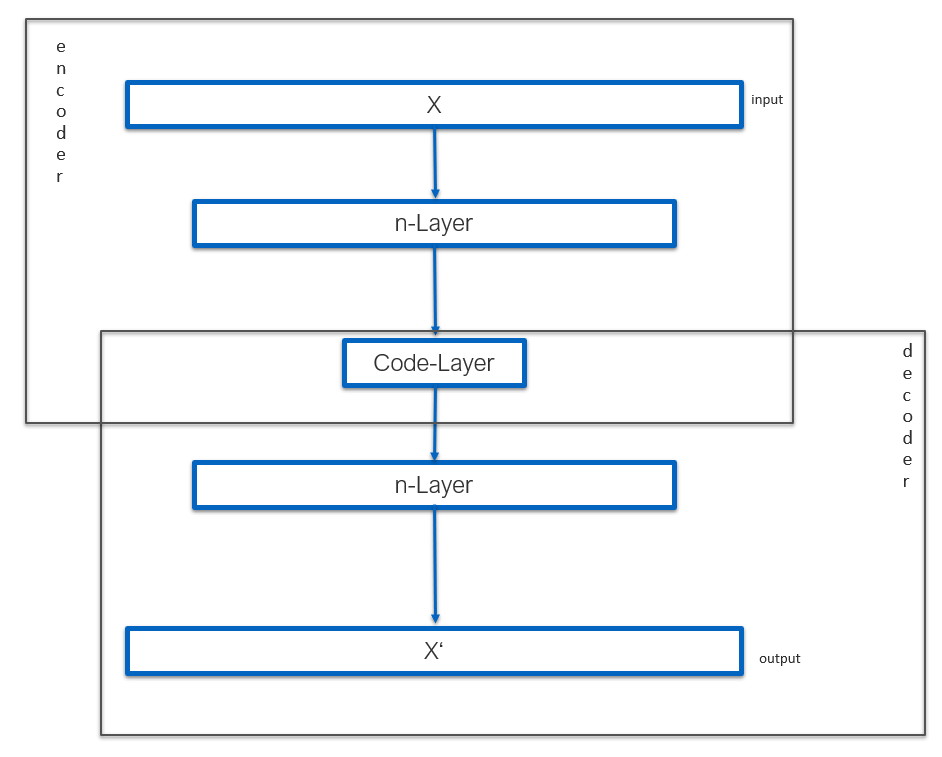
\includegraphics[width=0.7\textwidth, center]{bilder/Schema_Autoencoders/Schema_CAE2.png}
		\caption[Schema Autoencoder]{Schema eines Autoencoder}
		\label{img:SchemaCAE}
	\end{figure} 

	Der Encoder lässt sich vereinfacht als die Funktion $F(x)=c$ und der Decoder als die Funktion $ F(c)=x'$ darstellen, wobei $x\stackrel{!}{=}x'$ sein soll.
	 
	Autoencoder gibt es in vielen verschiedenen Ausführungen. Dabei sind die meisten Typen von Autoencoder unvollständige Autoencoder. Die verborgene Schicht, der Codelayer, enthält weniger Informationen als die Eingabe. Dadurch wird die Dimensionsreduzierung erzwungen. Andere Aufgaben können Entrauschung mittels Denoising-Autoencoder \cite{Vincent.2008} oder Generierung neuer Datenpunkte mittels Varrational-Autoencoder \cite{Kingma.2019} sein. Contractive-Autoencoder \cite{Rifai.2011} nutzen einen Regularisierer in der Zielfunktion, um das Modell zu zwingen eine Funktion zu lernen, die flexibler auf Variationen der Eingabewerte reagiert.   	

	Für diese Arbeit ist der \acl{cae} \cite{Masci.2011} kurz \ac{cae} interessant. Er ist ein Stacked-Autoencoder, welcher Faltungsschichten integriert. Faltungsschichten wurden in \cite{LeCun.1999} vorgestellt und haben sich in \cite{Krizhevsky.2012}, \cite{ChristianSzegedy.2014} und \cite{LeCun.2015} durchgesetzt. 
		
	\paragraph{Schichtenweise Vortrainieren} Im schichtenweise Vortrainieren \cite{Bengio.2007} werden einzelne Schichten eines neuronalen Netzwerkes vor dem eigentlichen Training vorbereitet, um die Leistung des gesamten Models zu erhöhen. Bei Autoencodern werden dabei die zueinander symmetrischen Schichten des Encoders und Decoders miteinander trainiert. Die Zielgröße ist dabei die Rekonstruktion der Eingabedaten.    

	\section{ Transferlernen}
	\label{sec:Transferlernen}
	Im traditionellen maschinellem Lernen wird pro Aufgabe und Datenset ein isoliertes Modell erstellt. Das Transferlernen wiederum hat das Ziel, Wissen zu teilen. Die Isolation der Modelle soll dabei aufgehoben werden. Dabei erfolgt eine Aufteilung in Quell- und Zieldomäne.
	
		\subsection{Tiefes Transferlernen}
		Geprägt durch die Entwicklung hin zu tiefen neuronalen Netzwerken wurden Methoden zum Tiefen Transferlernen vorgeschlagen. \cite{Tan.2018} ordnet diese in vier Kategorien ein. \\
		Der netzwerkbasierte Ansatz verwendet einen Teil des in der Quelldomäne trainierten Netzwerkes in der Zieldomäne wieder. Es werden dabei sowohl die Netzstruktur als auch die Verbindungsparameter übernommen. Die Netzwerke werden dabei in zwei Teile unterteilt. Der erste Teil ist die sprachunabhängige Merkmalstransformation, der zweite Teil ist der sprachabhängige Klassifikator. Dabei kann die sprachunabhängige Merkmalstransformation in der Zieldomäne wiederverwendet werden. Insbesondere in \cite{JasonYosinski.2014}, \cite{Long.2016} und \cite{George.2018} hat sich dieser Ansatz bewährt. Abgrenzend zu diesem Ansatz gibt es die Kategorie der instanzbasierten Ansätze. Diese ergänzen mittels fallspezifischer Strategie Gewichte in der Zieldomäne mit Gewichten aus der Quelldomäne. Abbildungsbasierte Ansätze, eine weitere Kategorie, bilden Instanzen aus der Quell- und Zieldomäne in einen neuen Datenraum ab. In diesem sind die Instanzen aus den zwei Bereichen ähnlich und können für ein gemeinsames Training eines tiefen neuronalen Netzwerkes genutzt werden. Die vierte Kategorie ist das Generative Adversarial deep Transfer Learning. Es ist von dem Ansatz Generative Adversarial Networks \cite{IanJ.Goodfellow.2014} inspiriert. Es werden übertragbare Repräsentationen gesucht, die sowohl auf die Quell- als auf die Zieldomäne anwendbar sind. \\
		Für eine Einordnung von klassischen Methoden des Transferlernens eignet sich die Erhebung \cite{FuzhenZhuang.2019}.
		 
		\subsection{Halbüberwachtes Lernen}
		Halbüberwachtes Lernen ist eine Methode, die sich zwischen unüberwachtem und überwachtem Lernen einordnen lässt. Die folgende Darstellung ist angelehnt an \cite{Chapelle.2010} . Methoden des unüberwachten Lernens arbeiten komplett ohne annotierte Daten, während überwachtes Lernen mit vollständig annotierten Daten arbeitet. Das halbüberwachte Lernen arbeitet mit teilweise annotierten Daten. Die Anzahl der nicht annotierten Daten übersteigt in der Regel die Menge der annotierten Daten. Diese Technik reduziert Annotationskosten durch den Einsatz weniger Daten mit Annotationen. Zu beachten ist dabei, dass sowohl die beschrifteten als auch die nicht beschriftete Daten aus der gleichen Verteilung entnommen werden. 
		Im Gegensatz dazu sind bei dem Transferlernen die Datenverteilungen der Quell- und Zieldomäne oft unterschiedlich.
				
		\subsection{Multi-Task-Learning}
		Werden mehrere Aufgaben parallel gelernt spricht man von dem \acl{mtl}, kurz \ac{mtl}. Der Begriff \ac{mtl} wurde insbesondere von \cite{Caruana.1998} geprägt. Ziel ist es, Wissen durch gleichzeitiges Lernen einiger verwandter Aufgaben weiterzugeben. Es wird davon ausgegangen, dass das Lernen einer Aufgabe das Lernen der anderen Aufgaben verbessert. Im Allgemeinen wird dies durch das Lernen aller Aufgaben gemeinsam erreicht, wobei die korrelierenden Informationen zwischen den einzelnen Aufgaben genutzt werden. Die Aufgaben erzeugen dabei eine niedrigdimensionale Repräsentation, welche dann durch das parallele Lernen besser generalisiert werden. In manchen Fällen hat sich zudem herausgestellt, dass \acl{mtl} zum Lernen von nicht verwandten Aufgaben vorteilhaft ist. \\
		Basierend auf den Ein- und Ausgängen wird \ac{mtl} von \cite{Thung.2018} in drei Fälle unterteilt. Der erst Fall wird  \acl{simo}, kurz \ac{simo} genannt. Diese Ansatz wird verwendet, um aus einer Eingabe Vorhersagen von verschiedenen Arten von Ausgabezielen zu treffen. Diese Art des \ac{mtl} wird auch \textit{multi-class learning} genannt. \acl{miso}, kurz \ac{miso} ist der Fall, dass mehrere Eingaben zum Vorhersagen eines Ausgabezieles genutzt werden.
		Die dritte Unterteilung wird \acl{mimo}, kurz \ac{mimo} genannt. Hierbei werden mehrere Eingaben zum Vorhersagen von verschiedenen Arten von Ausgabezielen genutzt.
		\begin{figure}[h]
			\centering
			\begin{subfigure}[c]{0.6\textwidth}			
				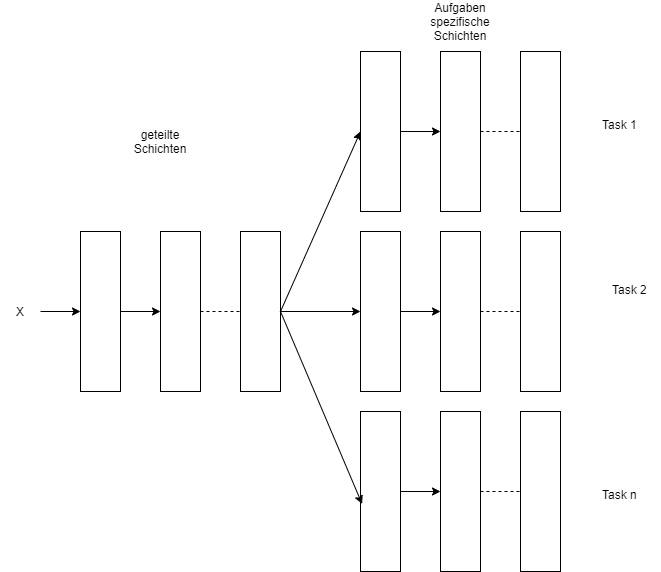
\includegraphics[width=1\textwidth, center]{bilder/Grundlagen/MTL/MTL_SIMO.png}
				\caption[MTL-SIMO]{Single-Input Multi-Output}
				\label{img:MTL_SIMO}	
			\end{subfigure}
			\begin{subfigure}[c]{0.49\textwidth}			
				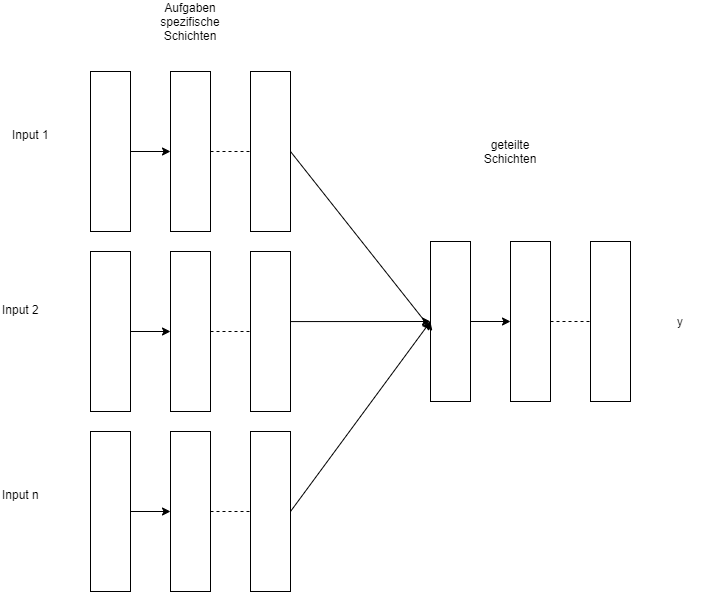
\includegraphics[width=1\textwidth, center]{bilder/Grundlagen/MTL/MTL_MISO.png}
				\caption[MTL-MISO]{Multi-Input Single-Output}
				\label{img:MTL_MISO}	
			\end{subfigure}
			\begin{subfigure}[c]{0.49\textwidth}			
				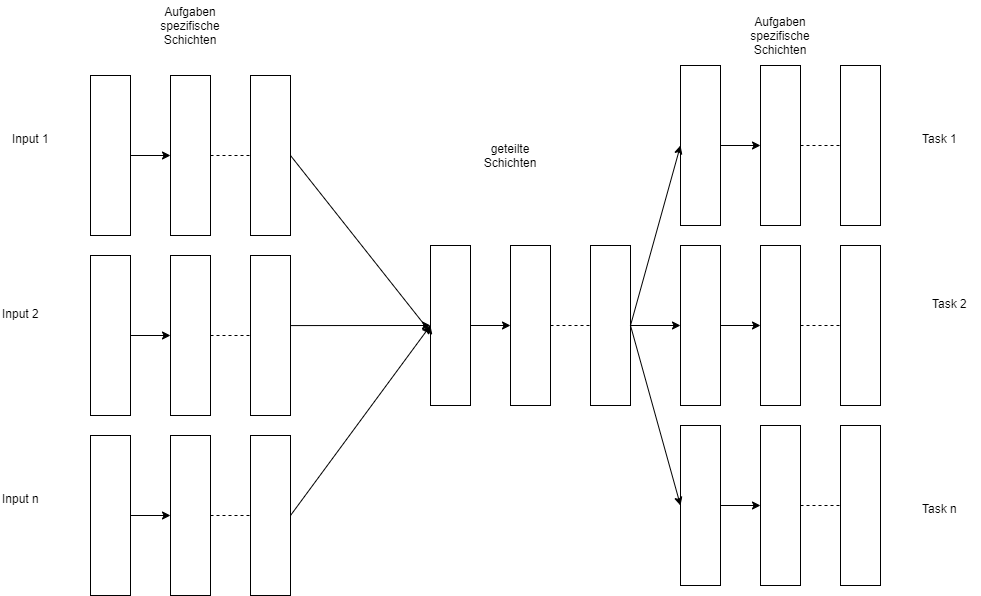
\includegraphics[width=1\textwidth, center]{bilder/Grundlagen/MTL/MTL_MIMO.png}
				\caption[MTL-MIMO]{Multi-Input Multi-Output}
				\label{img:MTL-MIMO}	
			\end{subfigure}
			\caption{Multi-Task-Learning: Ausprägungen}
			\label{img:MultiTaskLernen}
		\end{figure}
		Abbildung \ref{img:MultiTaskLernen} zeigt die verschiedenen Ausprägungen künstlicher neuronaler Netze, die auf \ac{mtl} beruhen.
		
		Induktives Transferlernen und \acl{mtl} wird darin unterschieden, dass beim induktiven Transferlernen angenommen wird, dass es eine Hauptaufgabe und eine Nebenaufgabe gibt. Die Nebenaufgabe bietet zusätzliche Informationen, um die Hauptaufgabe zu verbessern, bzw. zu generalisieren. Im \ac{mtl} gibt es keine solche Unterscheidung, die Aufgaben werden gleichberechtigt betrachtet. Induktives Transferlernen kann deshalb als Sonderform des \acl{mtl} gesehen werden. 
		
		Die Kombination von \acl{mtl} und Deep Learning für die Computervision wurde von \cite{YuchunFang.2017}, \cite{Li.2016}, \cite{RajeevRanjan.2016} und \cite{Zhao.2019} eingesetzt.

	\section{Automatisiertes maschinelles Lernen}
	\label{sec:AutoML}
  Automatisiertes maschinelles Lernen, kurz \ac{automl}, hat das Ziel, alle Aspekte des maschinellen Lernens und der Datenanalyse-Pipeline zu automatisieren. Die vollständige Automatisierung erlaubt es Nutzern ohne oder mit geringen Kenntnissen von ML-Techniken diese Systeme zu erstellen. Die vollständige Automatisierung ist ein langfristiges Ziel. Aktuelle Systeme sind halbautomatisch und zielen darauf ab, Personenaufwände durch Rechenvorgänge zu reduzieren. Trotz der steigenden Rechenleistung können AutoML-Methoden sehr rechenintensiv sein. Angelehnt an \cite{Hutter.2019} wird \ac{automl} in drei Methoden eingeordnet: Die \acl{hpo} kurz \ac{hpo}, das  Meta-Learning und \acl{nas} kurz \ac{nas}. 
	
	\subsection{\acl{hpo}}
	\label{subsec:HyperparameterOptimierung}	
	Angelehnt an \cite{Feurer.2019} sind Hyperparameter alle Parameter, welche vor Beginn des Trainings zur Steuerung des Trainings eingestellt werden können. Eine passende Einstellung dieser Parameter beeinflusst die Leistung eines Modells maßgeblich. In \cite{Kohavi.1995} wurde festgestellt, dass verschiedene Hyperparameterkonfigurationen für verschiedene Datensätze am besten funktionieren. Es ist also notwendig, für jede Aufgabe aufs Neue die beste Hyperparameterkonfiguration zu finden. Automatische \ac{hpo} ist die Technik des automatischen Findens der Hyperparameter, um die Leistung zu optimieren. Dabei hat sie insbesondere drei Ziele: An erster Stelle sollen Personenaufwände bei der Anwendung von maschinellem Lernen reduziert werden, zusätzlich soll es die Leistung von Algorithmen und Modellen des maschinellen Lernens verbessern. Ein weiteres Ziel ist es, die Reproduzierbarkeit von wissenschaftlichen Studien zu verbessern, da automatische \ac{hpo} einfacher reproduzierbar ist als manuelle \ac{hpo}. In Kapitel \ref{subsec:Optimierungstechniken} werden einige gängige Optimierungstechniken der automatischen \ac{hpo} erläutert. 	 
		
	\subsection{Meta-Learning}
	\label{subsec:MetaLearning}
	Unter \cite{JoaquinVanschoren.2018} ist eine Übersicht über das Meta-Learning zu finden. Meta-Learning umfasst jede Art von Lernen, welches auf frühere Erfahrungen zurückgreift. Dabei können umso mehr Arten von Metadaten genutzt werden, je ähnlicher die Aufgaben sind. Metadaten sind dabei alle Daten, die frühere Lernaufgaben beschreiben. Dies können z.B Algorithmuskonfigurationen, Hyperparameter, Netzarchitekturen und Modellbewertungen sein.
	
	\subsection{Neural Architecture Search}
	\label{subsec:NeuralArchitectureSearch}
	Im Deep Learning hängt die Leistung eines Modells maßgeblich von der genutzten Architektur ab. Das manuelle Suchen von Architekturen ist zeitaufwendig und fehleranfällig. Die Neural Architecture Search befasst sich damit, wie Architekturen automatisch gefunden werden können. Unter \cite{Elsken.2019} kann eine Übersicht über die Neural Architecture Search gefunden werden. 	

	\subsection{Optimierungstechniken}
	\label{subsec:Optimierungstechniken}
	In diesem Unterkapitel werden gängige Optimierungsmethoden des \ac{automl} dargestellt. Die Auflistung ist nicht vollständig, deckt aber die im praktischen Teil der Arbeit zur Verfügung stehenden Methoden ab.  
	
	\paragraph{Rastersuche}
	Die Rastersuche \cite{Michelucci.2018} ist eine modellunabhängige Optimierunsstrategie. Es werden Parameterkombinationen definiert, und anschließend werden, basierend auf den verwendeten Kombinationen, Modelle erstellt und evaluiert. \\ Schwachpunkt dieser Technik ist vor allem die notwendige Definition von Parameterkombinationen. Für jede Parameterkombination muss ein Modell trainiert und evaluiert werden. Wurde die optimale  Parameterkombinationen nicht definiert, kann sie nicht gefunden werden.
	 
	\paragraph{Zufallssuche}
	Die Zufallssuche ähnelt der Rastersuche. Sie unterscheidet sich dahingehend, dass die Parameterkombinationen nicht mehr definiert werden müssen. Es werden zufällige Stichprobenkonfigurationen aus dem definierten Parameterraum gezogen und evaluiert. In \cite{BergstraJamesandYoshuaBengio..2012} wurde gezeigt, dass insbesondere bei unterschiedlicher Wichtigkeit der Hyperparameter im Gegensatz zur Rastersuche bessere Ergebnisse erzielt werden. 

	\paragraph{Bayesian optimization}
	Nach \cite{Frazier.201807} ist Bayesian optimization ein Ansatz, der zur Optimierung von Zielfunktionen dient, die eine lange Zeit (Minuten oder Stunden) zur Auswertung benötigen. Im Gegensatz zur Rastersuche oder Zufallssuche ist der Ansatz modellabhängig. Der Ansatz ist iterativ und baut auf zwei Komponenten auf. Ein probabilistisches Ersatzmodell und eine Erfassungsfunktion, die zur Bewertung, welcher Punkt als nächstes bewertet werden soll, herangezogen wird. Das Ersatzmodell wird in jeder Iteration an alle Beobachtungen angepasst. Im Gegensatz zu modellunabhängigen Optimierungsmethoden, ist die Auswertung der Erfassungsfunktion billig und kann somit zur Optimierung herangezogen werden. 
	
	\paragraph{Successive Halving}
	\acl{sh} \cite{Jamieson.2015}, kurz \ac{sh}, weist einer Reihe von Hyperparameterkonfigurationen eine einheitliche Menge an Ressourcen zu, bspw. Zeit, Rechenleistung und modellspezifische Parameter, berechnet die Leistung von allen Konfigurationen und entfernt die schlechtere Hälfte. Die Konfigurationen werden dabei zufällig gezogen. Das Ganze wird wiederholt, bis eine Konfiguration übrig bleibt. In jedem Durchlauf werden der übriggebliebenen Hälfte exponentiell mehr Ressourcen zugewiesen. \ac{sh} benötigt als Eingangsparameter die Ressourcen und die Anzahl an Konfigurationen. Dabei muss abhängig vom Modell entschieden werden, ob wenige Konfigurationen mit mehr Ressourcen oder viele Konfigurationen mit weniger Ressourcen evaluiert werden sollen.
			
	\paragraph{Hyperband}	
	Hyperband \cite{Li.2017} erweitert \acl{sh}. Hyperband führt eine Rastersuche für die Parameter 'Ressourcen' und 'Anzahl Konfigurationen' durch. Es werden also mehrere \ac{sh}-Durchläufe mit diversen Konfigurationen durchgeführt. Die Anzahl an Konfigurationen wird dabei immer weiter reduziert. Abgeschlossen wird eine Ausführung mit einer Zufallssuche.
	
	\paragraph{BOHB}
	BOHB \cite{StefanFalkner.2018} ist ein Ansatz, der Bayesian optimization und Hyperband kombiniert. Dabei wird Bayesian optimization zur Auswahl von Konfigurationen herangezogen und Hyperband bestimmt, wie viele Konfigurationen mit welchem Ressourcen ausgeführt werden sollen. Anschließend werden die Konfigurationen mittels \acl{sh} ausgeführt. Unter https://github.com/automl/HpBandSter kann eine Implementierung des Werkzeuges gefunden werden. Diese Framework wurde für den praktischen Teil der Arbeit genutzt. 
			
	\section{Bibliotheken und Werkzeuge}
	\label{sec:BibliothekenundWerkzeuge}
	Für den praktischen Teil der Arbeit wurde insbesondere Cnvrg \cite{Kolben.2020} genutzt.\\
	Cnvrg.io ist eine 'full-stack' Data Science Platform, welche Werkzeuge für die Erstellung, Verwaltung, Bereitstellung und Automatisierung von maschinellem Lernen bereitstellt. Cnvrg.io erlaubt es, Arbeitsbereiche mittels Container zu erstellen. Die Container können dabei auf Maschinen in Azure \cite{MicrosoftCorporation.2020} zugreifen. Für die Experimente wurde ein vorgefertigter Container mit einer tesla-k80 \cite{Nvidia.2020}, fünf CPUs und 49 GB Arbeitsspeicher genutzt. 

	Für die Entwicklung wurden Python \cite{PythonSoftwareFoundation.2020}, Jupyter Notebooks \cite{ProjectJupyter.} und das Framework Tensorflow \cite{MartinAbadi.2015}  genutzt. Die wichtigsten Bibliotheken für die Arbeit sind Keras \cite{Chollet.2015} , Numpy \cite{Oliphant.2006} , Matplotlib \cite{Hunter.2007} , scikit-learn \cite{Pedregosa.2011} , ConfigSpace \cite{Lindauer.2019} , Bayesian Optimization and Hyperband \cite{StefanFalkner.2018}. 
	
	Für die Visualisierung von Bildeinbettungen wurde die Software 'PSIORI Visualizer' erweitert und eingesetzt. Die Software erlaubt es, dreidimensionale Daten darzustellen. Dabei können Filter eingesetzt sowie Blickwinkel geändert werden. Daten können mit zusätzlichen Informationen versehen werden und Zoomen ist möglich. Als zusätzliche Information können z.B. ein Originalbild und seine Rekonstruktion oder die Information, ob eine Vorhersage korrekt oder falsch war, hinterlegt werden.
	
	Kern der erstellten Softwaremodule ist das Framework Psipy \cite{PSIORIGmbH.2019}. Psipy ist ein Python-Framework für maschinelles Lernen, das von PSIORI selbst entwickelte Werkzeuge zusammenfasst und unter einer einheitlichen API zu Verfügung stellt. Diese API ist an die API des verbreiteten Frameworks scikit-learn angelehnt. Es können Modelle basierend auf scikit-learn  und Tensorflow eingebunden werden. In den nachfolgenden Abschnitten werden die wichtigsten bestehenden Module des Frameworks vorgestellt.
	
	 \paragraph{saveable.py} Das Modul \textit{saveable} ist eine flexible Basisklasse, die Kernfunktionalität zum Speichern und Laden von Python-Objekten bietet. Modelle, die verschiedene Bibliotheken nutzen, können so einheitlich gespeichert werden. Um die Klasse \textit{Saveable} nutzen zu können, müssen erbende Klassen ihre Konstruktorargumente an die Basisklasse übergeben. Zusätzlich ist es notwendig, eine Erweiterung beim Speichern und Laden zu implementieren. Beim Speichern ist es notwendig, eine Erweiterung um alle Module und weitere Argumente zu implementieren. Beim Laden müssen die gespeicherten Module und Argumente geladen werden. In Listing \ref{lst:SaveTensorflow} ist die Erweiterung zum Speichern eines Tensorflow-Models abgebildet. \\
	 \\
	\begin{lstlisting}[language=python,caption=Erweiterung zum Speichern eines Tensorflow Models, label=lst:SaveTensorflow]
		...
		zip_file.add("model.h5", self.model)
		...
	\end{lstlisting}

	\paragraph{autoencoder.py} Das Modul \textit{autoencoder} enthält die drei Klassen \textit{StackedAutoencoder}, \textit{FullyConnectedAutoencoder} und \textit{ConvolutionalAutoencoder}. \\	
	Der \textit{StackedAutoencoder} wird als Basisklasse für die anderen beiden Klassen genutzt. Im Konstruktor werden Methoden aufgerufen, die in den abgeleiteten Klassen ausprogrammiert sind. Dabei wird ein Keras-Modell für einen Encoder und Decoder entsprechend von Parametern erstellt. Als weitere wichtige Methoden gibt es die Methode $pretrain(..)$ und $fit(..)$. Mittels $pretrain(..)$ werden die Schichten eines symmetrischen Autoencoder von außen nach innen, wie in \cite{Bengio.2007} beschrieben, vortrainiert. Die Zuordnung der Schichten erfolgt in den abgeleiteten Klassen.
	In der $fit(..)$-Methode wird nach einigen Prüfungen die Methode f$fit(..)$ \cite{Chollet.2015} des Kerasmodels aufgerufen. In Abbildung \ref{img:KlassendiagrammConvolutionalAutoencoder} ist das Klassendiagramm mit den öffentlichen Methoden des ConvolutionalAutoencoder dargestellt. 
	\begin{figure}[h]
		\centering
		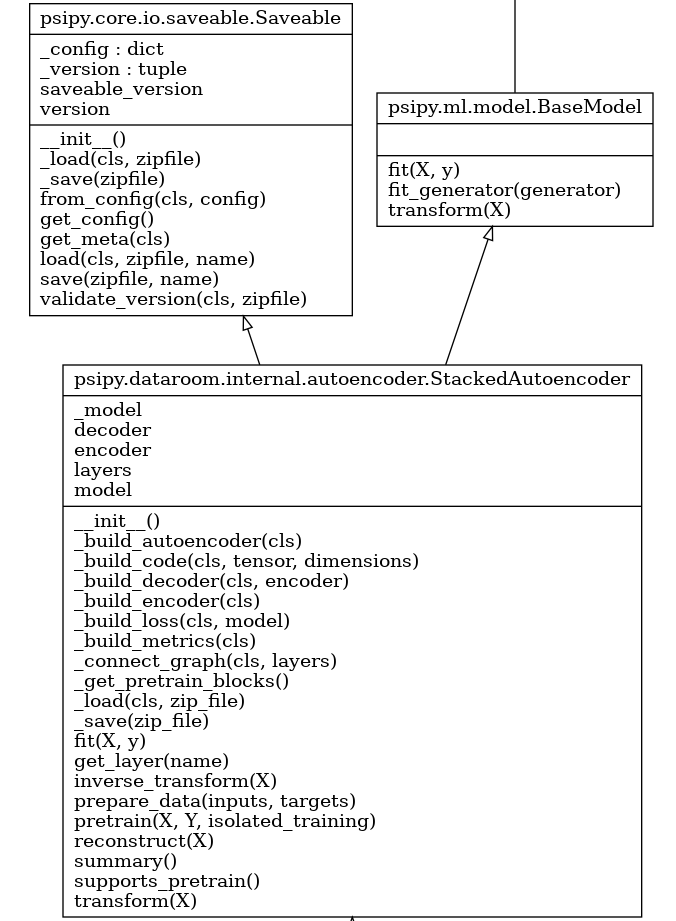
\includegraphics[width=0.6\textwidth, center]{bilder/Klassendiagramme/klassendiagramm_public_cae2.png}
		\caption[Klassendiagramm ConvolutionalAutoencoder]{Klassendiagramm ConvolutionalAutoencoder}
		\label{img:KlassendiagrammConvolutionalAutoencoder}
	\end{figure}  
	
	\paragraph{hyperparameter\_mixin.py}  \textit{Hyperparameter\_mixin} wird zum standardisierten Verwalten von Hyperparametern für AutoML-Klassen genutzt. Auf die Hyperparameter kann anschließend einheitlich zugegriffen werden. Abbildung \ref{img:KlassendiagrammHyperparametermixin} zeigt das zugehörige UML-Klassendiagramm mit den Methoden zum Hinzufügen, Löschen und Laden der Hyperparameter. Da die Methoden öffentlich sind, können über jede erbende Klasse die Hyperparameter eigenständig verwaltet werden.	
	\begin{figure}[h]
		\centering
		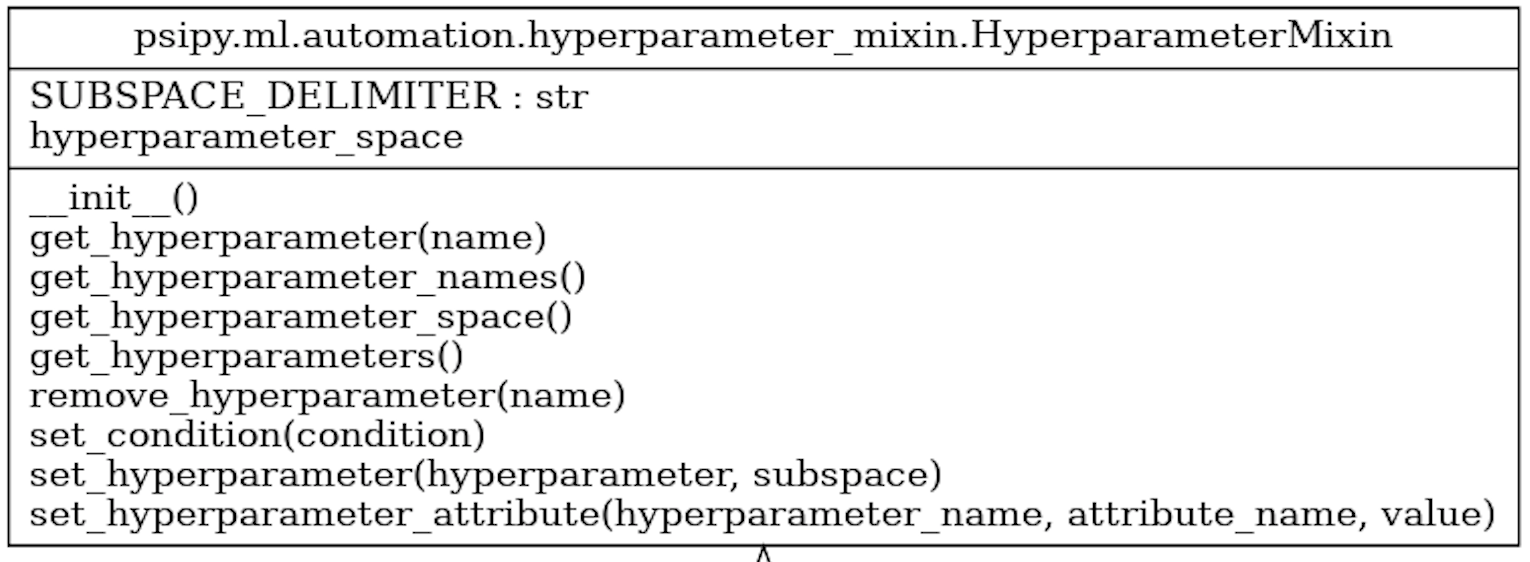
\includegraphics[width=0.6\textwidth, center]{bilder/Klassendiagramme/Hyperparametermixin.png}
		\caption[Klassendiagramm Hyperparametermixin]{Klassendiagramm Hyperparametermixin}
		\label{img:KlassendiagrammHyperparametermixin}
	\end{figure}  
	
	\section{Einordnung und bestehende Systeme}
	\label{sec:BestehendesSystem}
	Die Bilddaten und Aufgabenstellungen der neuronalen Netzwerke sind in die Problemstellungen des Autocrane-Projekts \cite{PSIORIGmbH.2020} von PSIORI einzuordnen. Es sind echte Datensätze und echte Problemstellungen, wobei die gezeigten Aufgabenstellungen und Modelle nicht zwingend in dem Autocrane-Projekt zum Einsatz kommen. Das Autocrane-Projekt ist ein laufendes Projekt, welches das Ziel hat, einen feststehenden Rundlaufkran vollautomatischen zu steuern. In Abbildung \ref{img:CircularCrane} ist ein Rundlaufkran abgebildet. Diese Art von Kran wird in holzverarbeitenden Anlagen zum Befüllen von Fülltrichtern oder Förderbändern eingesetzt. Der Kran kann sich um 360 Grad drehen. Der Greifer kann nach oben, unten und mittels eines Schlittens entlang eines Auslegers bewegt werden. Um die Bilder aufnehmen zu können, wurde an der Kabine am Hauptstandfuß eine Kamera angebracht. Die Kamera ist auf das Ende des Auslegers und den Bereich darunter ausgerichtet. Die Kamera bewegt sich mit dem Rundlaufkran, wodurch der Greifer immer im Bild ist. Für das Autocrane-Projekt sind insbesondere drei Anwendungsfälle interessant. Die Baumstämme werden mittels LKW angeliefert und müssen nach vorgegebenen Regeln (z. B. Ausrichtung, freier Lagerplatz) als Holzstapel gelagert werden. Der Fülltrichter kann mit Holz aus den Holzstapel oder mit Holz aus einem LKW befüllt werden. Es ergeben sich Aufgabenstellungen wie Greifer-Erkennung, Baumstamm-Erkennung, LKW-Erkennung, Strategien für das Entladen und Aufbewahren der Baumstämme und weitere Aufgaben. Im Normalbetrieb werden täglich 140-200 LKW entladen. Die Ladung ist 9 - 18 Meter lang und 34 - 40 Tonnen schwer. 
	\begin{figure}[h]
		\centering
		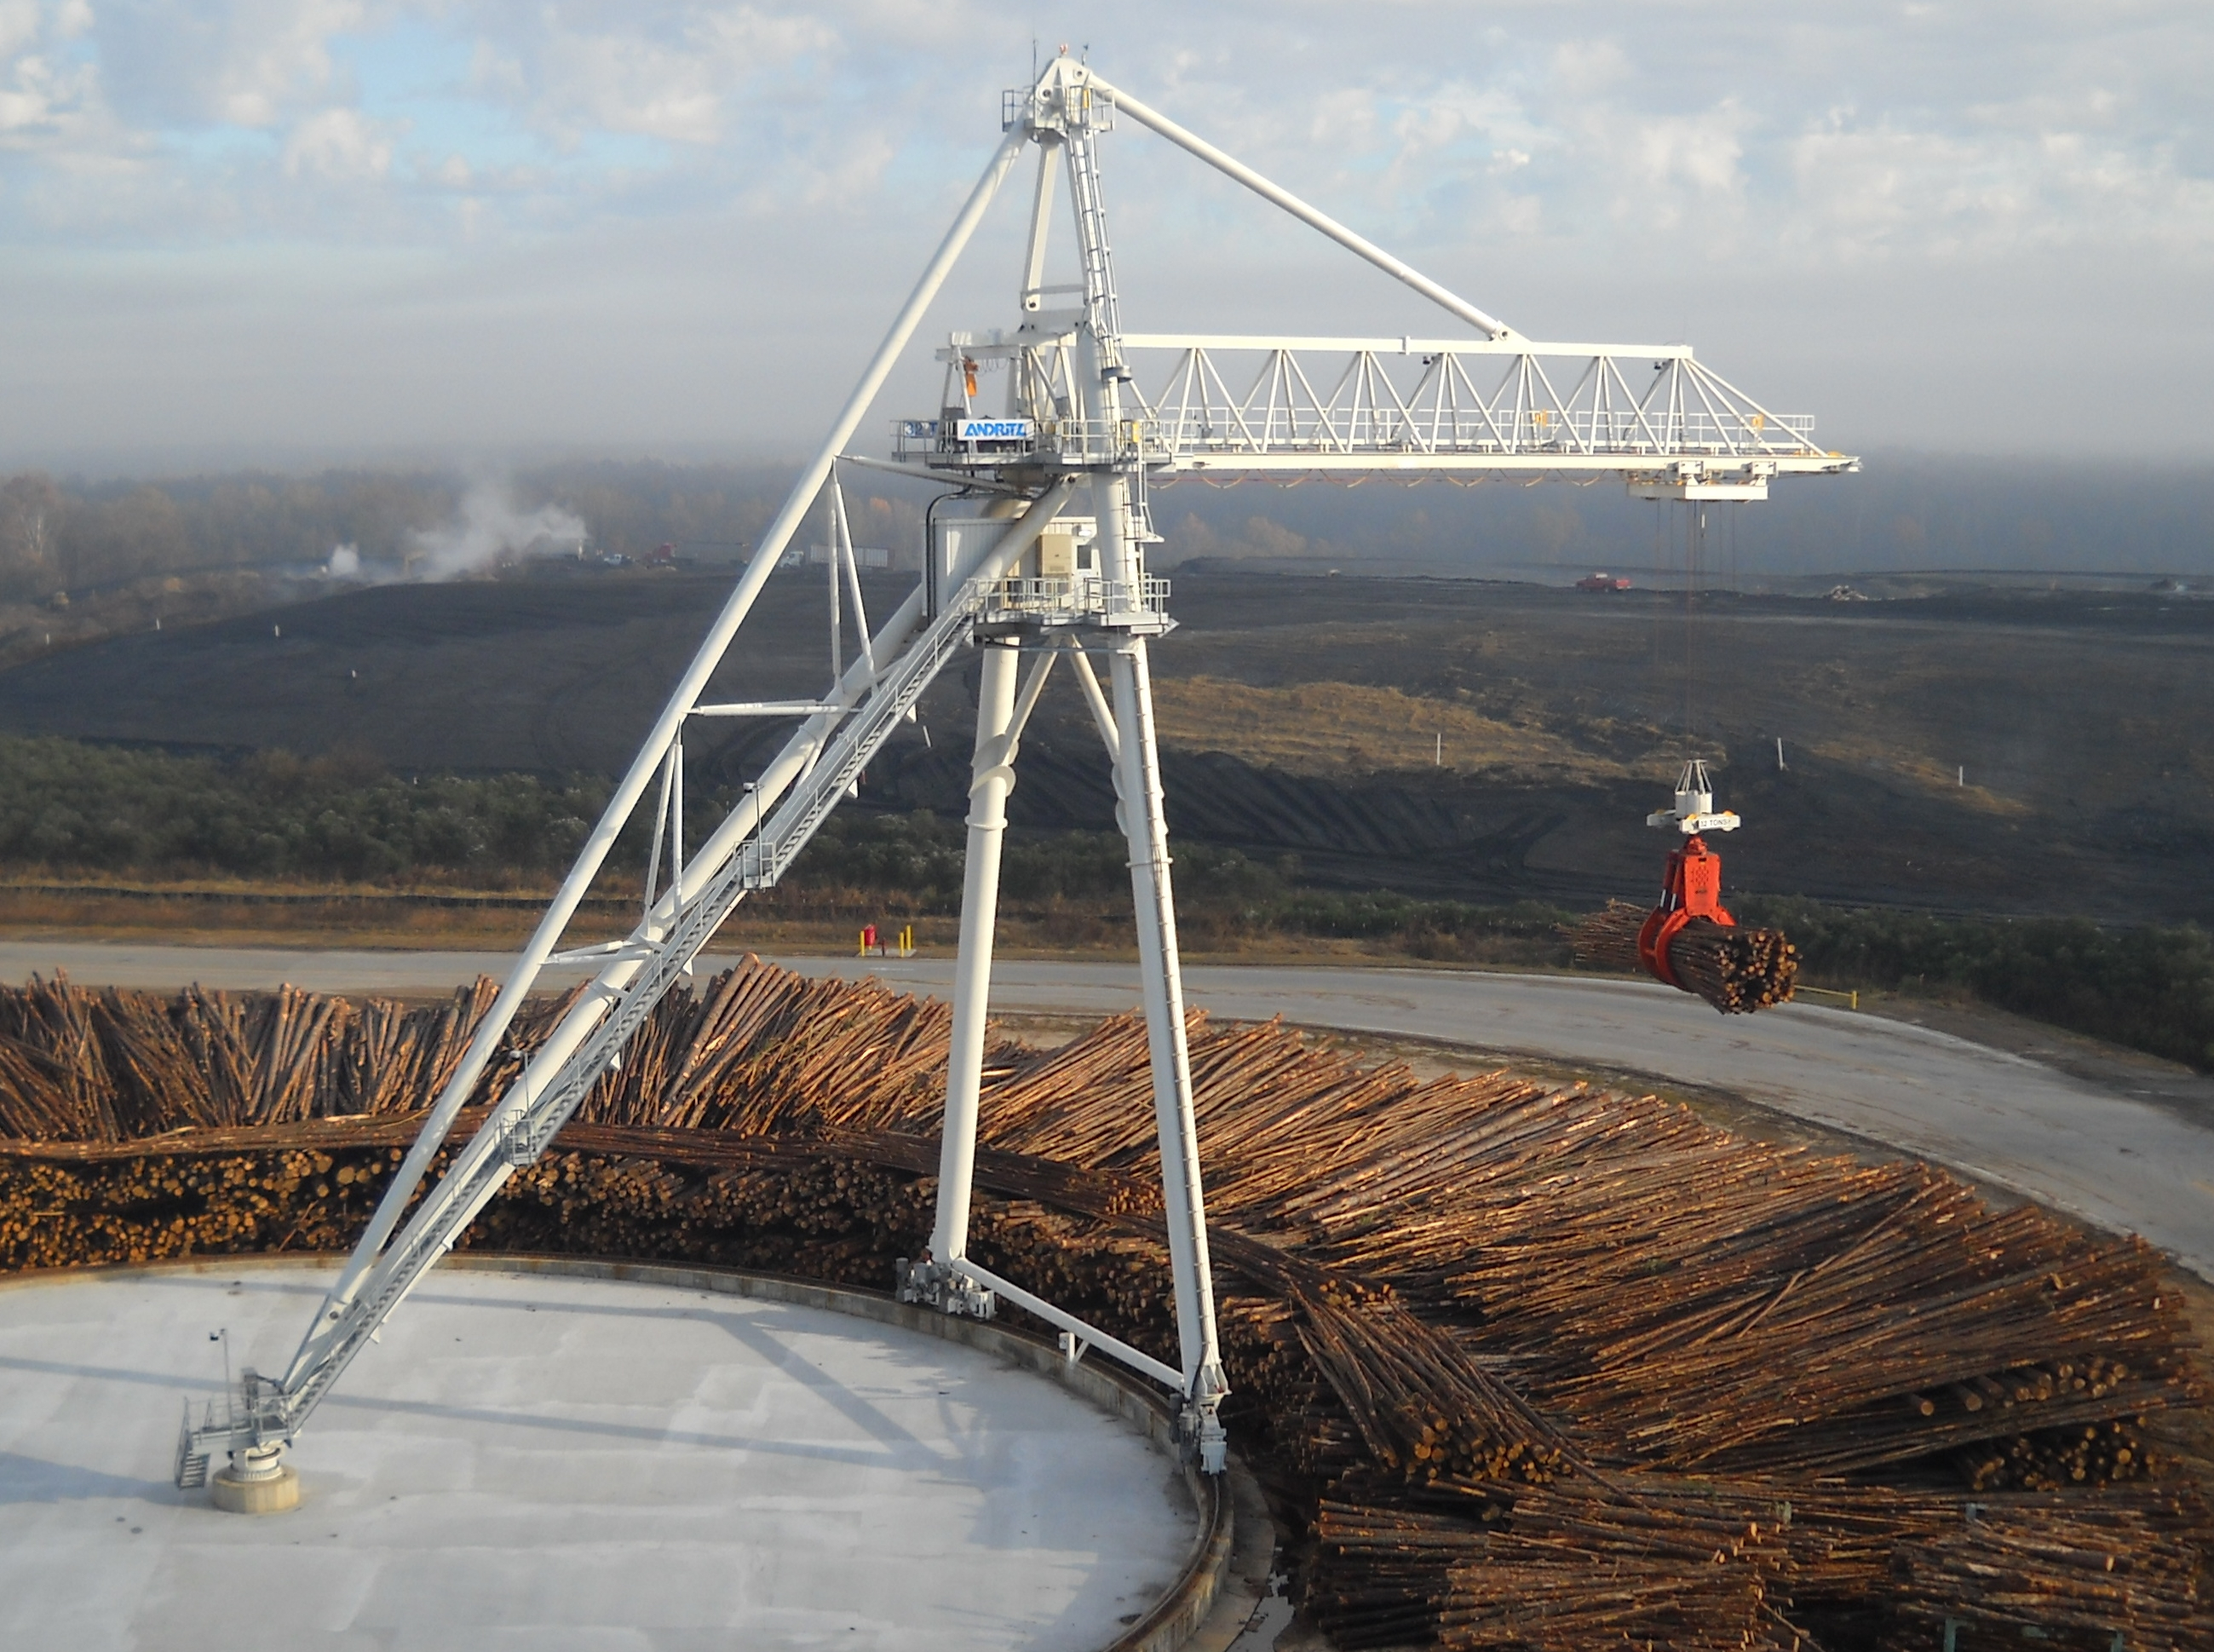
\includegraphics[width=0.5\textwidth, center]{bilder/Grundlagen/Kran_vollstaendig_N1_030.jpg}
		\caption[Rundlaufkran]{Rundlaufkran (Foto: ANDRITZ)}
		\label{img:CircularCrane}
	\end{figure}		

	\paragraph{Greifererkennung} Bei der Aufgabenstellung muss in einem Bild die Position eines Rahmen um den Greifer gefunden werden. Abbildung \ref{img:Grapple} zeigt ein Bild eines Rahmens um den Greifer. Es handelt sich um eine klassische Objekterkennungs-Aufgabe.
	\begin{figure}[h]
		\centering
		\begin{subfigure}[c]{0.49\textwidth}			
			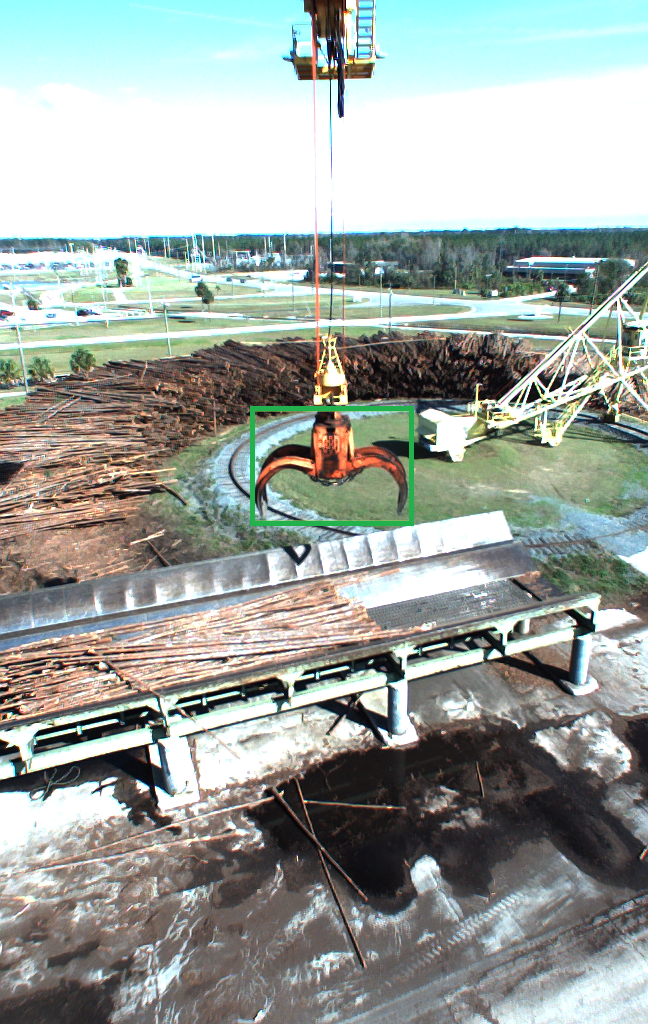
\includegraphics[width=1\textwidth, center]{bilder/Grundlagen/Grapple2.png}
			\caption[Bsp. Bild: Greifer mit Rahmen]{Greifer mit Rahmen}
			\label{img:Grapple}	
		\end{subfigure}
		\begin{subfigure}[c]{0.49\textwidth}			
			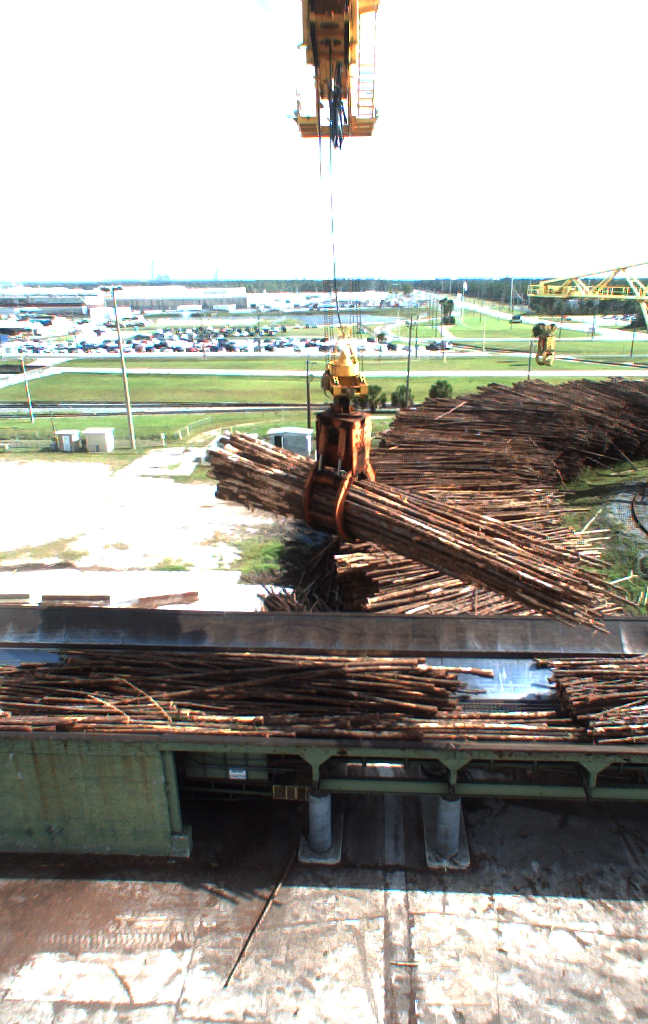
\includegraphics[width=1\textwidth, center]{bilder/Grundlagen/Logs_14.png}
			\caption[Bsp. Bild: Greifer mit Baumstämmen]{Greifer beladen}
			\label{img:Logs}	
		\end{subfigure}
		\caption{Greifer}
		\label{img:Greifer}
	\end{figure}	
	PSIORI hat die Aufgabe mittels neuronalem Netzwerk gelöst. Dabei wurde auf die Technik des \acl{ssd} \cite{Liu.2015}, kurz \ac{ssd},  zurückgegriffen. Die Vorhersagegenauigkeit dieses Modells wird als Basislinie und Vergleichswert genutzt. Dabei ist die ausschlaggebende Metrik die \acl{iou}, kurz \ac{iou}. Mit einem Schwellenwert von $>= 0.8$ wird eine Einteilung in korrekt vorhergesagte Rahmen durchgeführt. Es wird also die Fläche der Überschneidung der beiden Rahmen durch die Gesamtfläche der Rahmen geteilt und wenn ein Wert $>= 80\%$ erreicht wird, als korrekt vorhergesagt eingestuft. Das Modell erreicht einen Wert von $0.86$. In Anhang \ref{appendix:BasislinieGreifer} ist die vollständige Basislinie dargestellt.
	
	\paragraph{Greifer beladen?} Die Aufgabe 'Greifer beladen?' hat zum Ziel, zu erkennen ob sich Baumstämme im Greifer befinden oder nicht. Es handelt sich um eine Klassifikationsaufgabe. Für diese Aufgabe wurde von PSIORI ein Modell erstellt. Dieses Modell wird wie das Greifererkennungsmodell als Basislinie und Vergleichswert für die durchgeführten Versuche genutzt. Das Modell erreicht auf den Validationsdaten eine \textit{Accuracy} von 98.28\%. Im Anhang \ref{appendix:BasislinieBaumstämme} ist die vollständige Basislinie dargestellt. 

	\section{Datenverständnis}
	\label{sec:DataUnderstanding}
	Mittels Kamera an der Kabine können neue unbeschriftete Bilder aufgenommen und bei PSIORI abgelegt werden. Durch den Aufbau des Rundkrans und der Kameraposition, befindet sich der Greifer immer im Bild. Der Hintergrund der Bilder ändert sich stark. Die geografische Lage des Rundkrans schränkt die möglichen Wetterlagen ein. Es fällt kein Schnee und es gibt wenige Regentage. In Abbildung  \ref{img:Bildqualität} sind Ausprägungen der Bildqualität dargestellt. Abgesehen von Bildern in guter Qualität gibt es helle Bilder, dunkle Bilder und Bilder mit Reflexionen. Die Bilder sind 1024 auf 648 Pixel groß und in Farbe. Die einzelnen Pixel, pro Farbkanal können dabei Werte zwischen 0 und 255 annehmen. 
	Entsprechend der beiden Aufgabenstellungen 'Greifererkennung' und 'Greifer beladen' werden Daten mit einer passenden Beschriftung bereitgestellt.	
	\begin{figure}[h]
		\centering
		\begin{subfigure}[c]{0.24\textwidth}			
			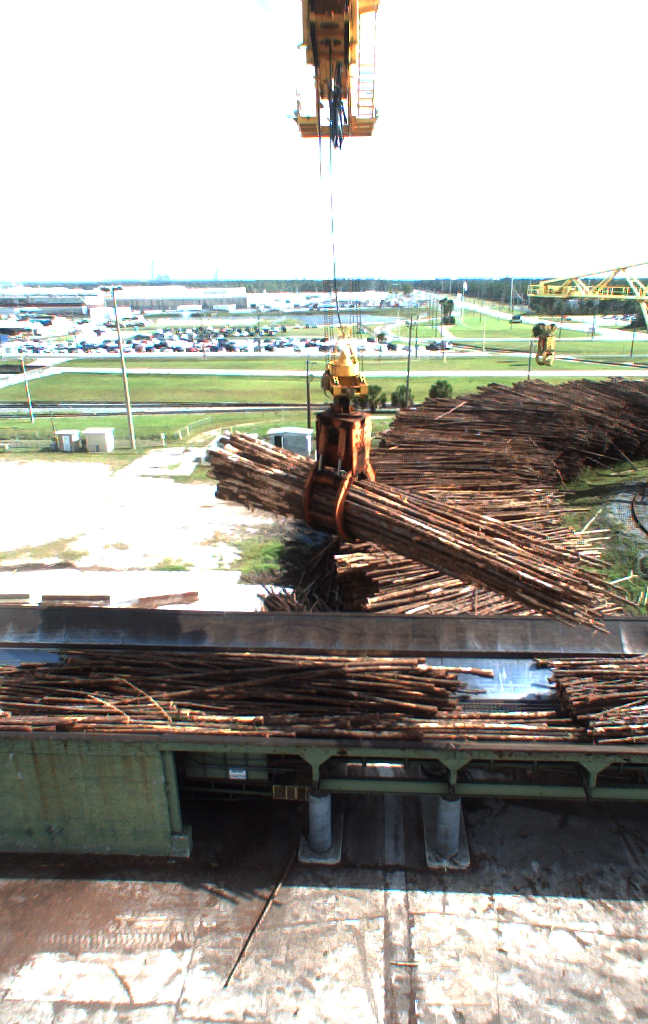
\includegraphics[width=1\textwidth]{bilder/Grundlagen/Logs_14.png}%{bilder/Grundlagen/Daten_Bildqualitaet/gut.png}
			\subcaption{Gut}			
		\end{subfigure}
		\begin{subfigure}[c]{0.24\textwidth}			
			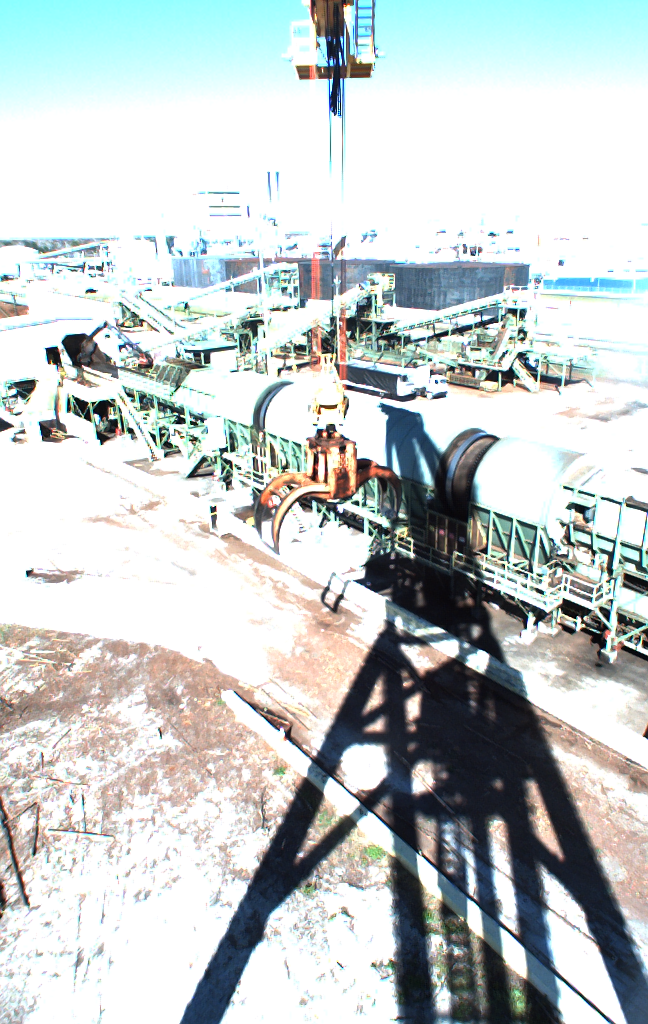
\includegraphics[width=1\textwidth]{bilder/Grundlagen/Daten_Bildqualitaet/hell_schatten.png}
			\subcaption{Hell}			
		\end{subfigure}
		\begin{subfigure}[c]{0.24\textwidth}			
			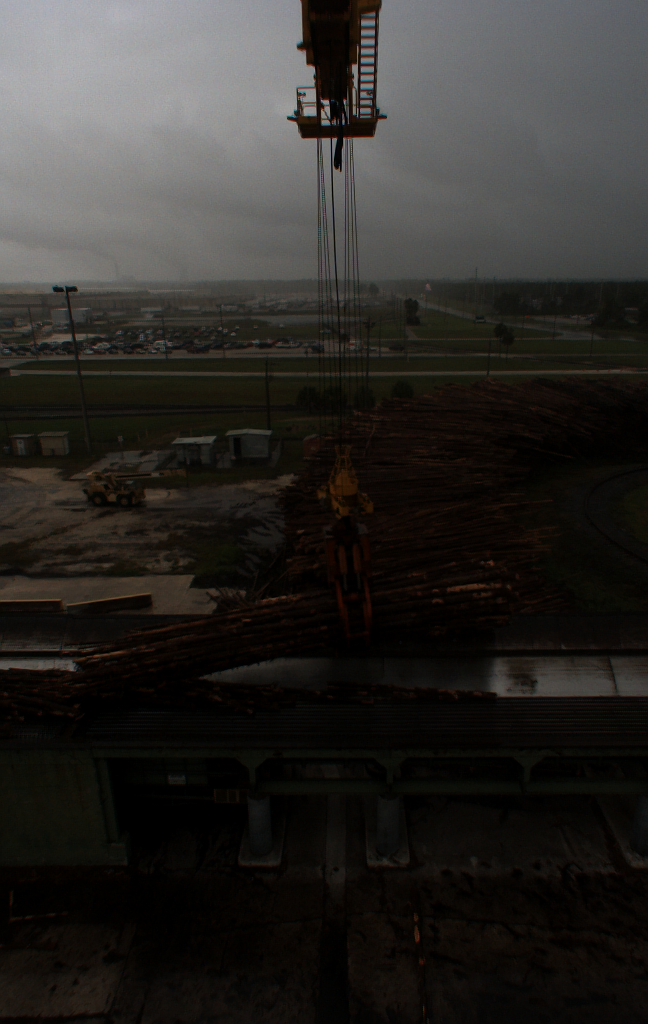
\includegraphics[width=1\textwidth]{bilder/Grundlagen/Daten_Bildqualitaet/dunkel.png}
			\subcaption{Dunkel}			
		\end{subfigure}
		\begin{subfigure}[c]{0.24\textwidth}			
			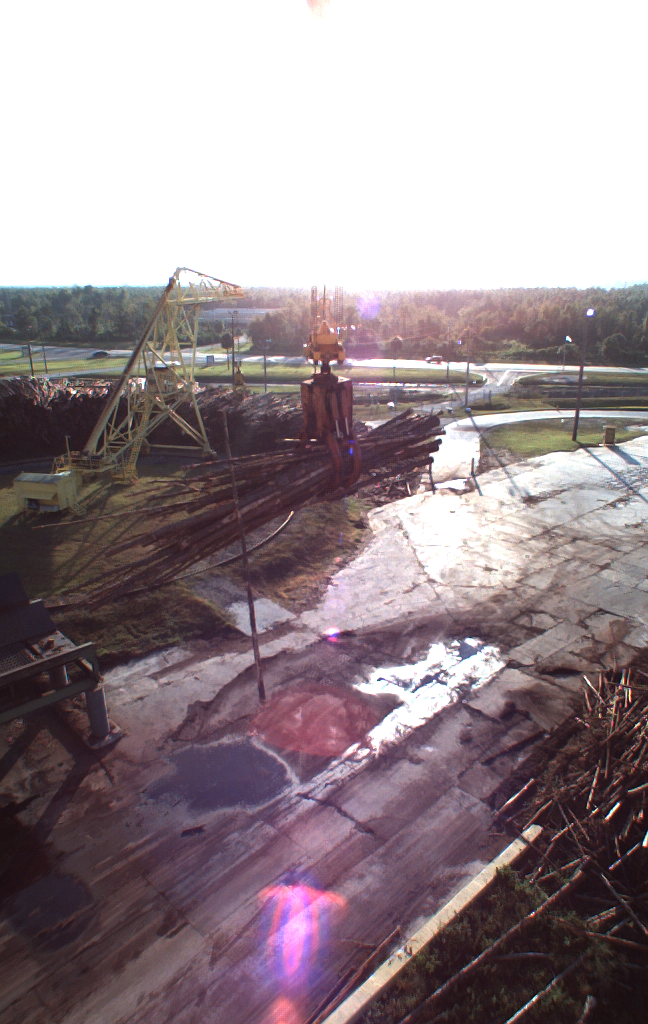
\includegraphics[width=1\textwidth]{bilder/Grundlagen/Daten_Bildqualitaet/Reflexionen.png}
			\subcaption{Reflexionen}			
		\end{subfigure}
		\caption{Bildqualität}
		\label{img:Bildqualität}
	\end{figure}
		
	\paragraph{Greiferdatensatz} Der Greiferdatensatz enthält Bilder, in welchen der Greifer mittels Rahmen markiert ist. Abbildung \ref{img:Grapple} zeigt ein beispielhaftes Bild mit markiertem Greifer. Die Annotationen der Position des Greifers wurde pro Bild in einer XML-Datei abgelegt. Konkret wurde die Position des Rahmens in der Form ymin, xmin, ymax und xmax abgespeichert. Über die vier Werte lässt sich problemlos ein Rahmen um den Greifer spannen. Der Datensatz besteht aus 4.684 durch Personen annotierten Bildern.
	
	\paragraph{Generierter Greiferdatensatz} Erfahrungsgemäß lernen Autoencoder Lichtverhältnisse in Bildern relativ gut. Um für erste Versuche den Fokus von den Lichtverhältnissen auf die eigentliche Aufgabenstellung zu setzen, wurde ein weiterer Greiferdatensatz erzeugt. Hierfür wurden 8963 Bilder mittels dem Basislinienmodell beschriftet und in 7171 Trainingsdaten und jeweils 896 Test- und Validationsdaten aufgeteilt.
	 
	\paragraph{Baumstammdatensatz} Der Baumstammdatensatz enthält Bilder, welche die Annotation, ob sich Baumstämme im Greifer befinden oder nicht, enthält. Die Bilder sind durch zwei Ordner in Bilder mit und Bilder ohne Baumstämme aufgeteilt. Abbildung \ref{img:Logs} zeigt ein Bild, in welchem der Greifer Baumstämme greift. In Abbildung \ref{img:Grapple} befinden sich keine Baumstämme im Greifer.  
			
	\section{Datenvorbereitung}
	\label{sec:DataPreparation}
	In Vorbereitung auf die Modellierungsphase wurde ein finaler Datensatz erstellt und Werkzeuge zum Laden und Vorbereiten der Daten implementiert.
	\paragraph{Erste Iteration} Als Erstes wurden die Daten mittels Skripte in Training-, Test- und Validationsdaten aufgeteilt. Anschließend wurden die Daten auf der Cnvrg-Plattform in einen versionierbaren Datenspeicher geladen. In Tabelle \ref{table:DatenaufteilungTrainTestValidation} ist die finale Datenaufteilung zu sehen. Die Greiferdaten sind in 70\% Trainingsdaten und jeweils 15\% Test- und Validationsdaten aufgeteilt. Die Baumstammdaten sind in 80\% Trainings-, 10\% Test- und 10\% Validationsdaten getrennt worden. Die Trainingsdaten werden zum Trainieren der Modelle genutzt, die Testdaten zum Überprüfen der Modelle und die Validationsdaten werden am Ende der Experimente für die finale Überprüfung der Ergebnisse eingesetzt.
	\begin{table}[ht]
		\centering
		\begin{tabularx}{\textwidth}{lllll}
			& \textbf{Train} & \textbf{Test}  & \textbf{Validation} & \textbf{Summe} 	 \\
			\textbf{Greifer} 				 & 	3.279			& 703	 & 704				   & 4.686 	\\
			\textbf{Baumstämme j/n}	 	  &  9.749	   & 1.221 	& 1.225	& 12.195\\		
		\end{tabularx}
		\caption{Datenaufteilung - Train Test Validation}
		\label{table:DatenaufteilungTrainTestValidation}
	\end{table}
	
	Für das Laden der Daten wurde das Modul \textit{data\_loader.py} erstellt. Dieses Modul enthält die drei Klassen \textit{DataLoader}, \textit{GrappleDataLoader} und \textit{LogsDataLoader}. \textit{DataLoader} ist eine abstrakte Klasse, die Methoden zum Laden der Trainings-, Test- und Validationsdaten definiert. \\ 
	Sie liefern die Bilder basierend auf einem Parameter bis zur maximalen Anzahl als Numpyarray zurück. Die Klassen \textit{GrappleDataLoader} und \textit{LogsDataLoader} implementieren für den jeweiligen Datensatz die konkreten Methoden zum Laden der Daten. \\
	Mittels des Moduls \textit{data\_preparation.py} und der Klasse \textit{Preprocessing} werden die Bilder auf die passende Größe verkleinert oder vergrößert und auf den Wertebereich zwischen 0 und 1 normalisiert.
	
	\paragraph{Zweite Iteration} 
	In der zweiten Iteration wurde ein neues Modul namens \\ \textit{data\_generator\_provider.py} erstellt. Da Bilder als Numpyarray direkt in den Speicher geladen werden, können nicht beliebig viele Bilder genutzt werden. Dieses Problem wird von den Keras \textit{ImageDataGeneratoren} \cite{Chollet.2015} adressiert. Sie erlauben es Bilder stapelweise bereitzustellen. Zusätzlich können die \textit{ImageDataGeneratoren} die Bilder direkt in der benötigten Größe bereitgestellt werden. Das Modul implementiert jeweils für den Baumstammdatensatz und den Greiferdatensatz eine Klasse zum Bereitstellen von \textit{ImageDataGeneratoren}.
	
	Da die Modelle \ac{simo}-Modelle sind, erfolgt zusätzlich noch eine Aufbereitung der Bereitstellung der Daten. Standardmäßig stellen die Generatoren Stapel mit Einträgen der Form $X ,Y$  bereit. Wobei X die Eingangsdaten sind und Y die Zielgröße definiert. Zum Beispiel kann X ein Bild sein und Y die zugehörige Klasse. Die Multi-Task-Learning-Module benötigen Generatoren, die Einträge der Stapel der Form $X, [X, Y]$ erzeugen. Die Zielgröße hat sich zu einer Liste mit zwei Größen verändert. Die erste Zielgröße entspricht den Eingangsdaten, sie werden für den Decoder-Ausgang genutzt. Die zweite Zielgröße wird für den zweiten Ausgang genutzt. Sie entspricht der Zielgröße eines normalen \textit{ImageDataGenerator}. Das Ganze wird mit Hilfe der Klasse \textit{tensorflow.keras.utils.Sequence} erreicht. Ihr wird im Konstruktor ein \textit{ImageDataGenerator} übergeben. Bei der Bereitstellung eines Elementes wird der Rückgabewert des Generators angepasst. Die entscheidenden Codezeilen sind in Listing \ref{lst:AufbereritungGeneratorergebnis} dargestellt. 
	\begin{lstlisting}[language=python,caption=Aufbereitung Generatorergebnis in Python, label=lst:AufbereritungGeneratorergebnis]
		res = self.generator.next()
		return res[0], [res[0], res[1]]
	\end{lstlisting}
	
	Für das Vortrainieren werden Generatoren bereitgestellt, welche Stapel mit Einträgen der Form $X ,X$ erzeugen. Hierbei wird auf Standardfunktionalität der Klasse \textit{ImageDataGeneratoren} zurückgegriffen. \\
	Die \textit{ImageDataGeneratoren} bieten Standardfunktionalität zur Bildverstärkung. Alle Generatoren normalisieren die Werte der Bilder zwischen 0 und 1. Die Generatoren für die Trainingsdaten führen noch zufällige Veränderungen der Helligkeit und Kanalverschiebungen durch. Bei den Baumstammdaten werden die Bilder zusätzlich horizontal umgedreht. 


 


 
